\subsection{System Definition}\label{subsec:system-definition}

The system definition, as per definition, is
\textcquote[23]{mathiassen2018}{[a] concise description of a computerized system expressed in natural language.}
Such a definition serves as the basis of any further procedures, due to it giving a specific perspective on the problem
at hand.
After consultations with the client, and the process of gaining deep, objective insight into the issues through the
consideration of different ideas, all the involved parties agreed upon one specific perspective.
The system definition that can be found down below attempts to reflect this perspective in a manner that can be
understood by everyone involved.
Furthermore, the definition also involves the interpretation of the system as stated through the statement earlier in
Section~\ref{subsec:problem-statement}.

% textidote: ignore begin
\begin{figure}[H]
    \centering
    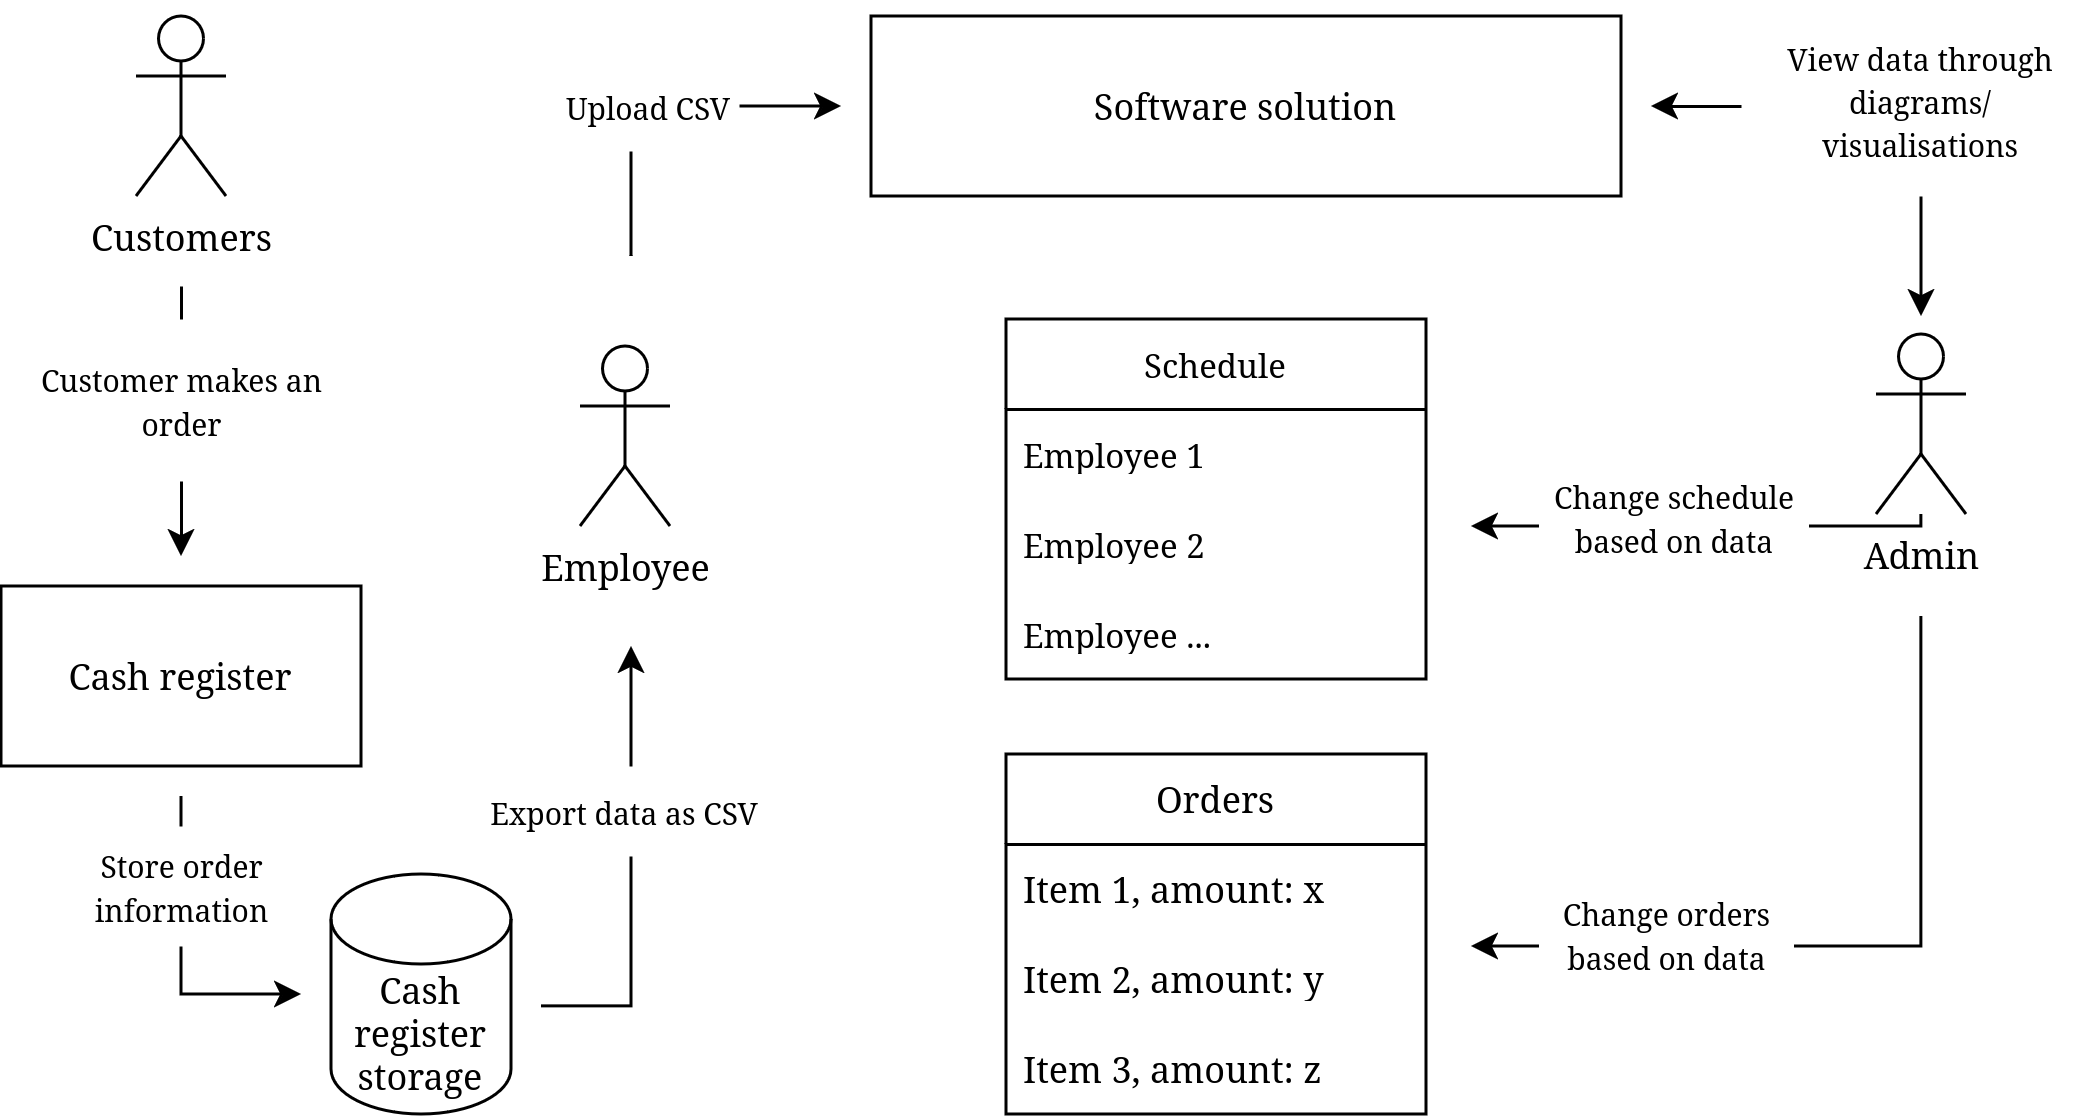
\includegraphics[width=\textwidth]{rich_pictures_solution}
    \caption{A rich picture visualizing the proposed solution}\label{fig:pda-solution}
\end{figure}
% textidote: ignore end

Because system definitions also should reflect specific limitations~\cite[38]{mathiassen2018}, the group decided to
limit the system in terms of a specific user experience, target group, and system objective, rather than creating a
generalized system that also covers the client's needs.

Taking into consideration all the alternatives that were weighed, the following system definition was coined:
\begin{tcolorbox}[title=System definition]
    The digital system should enable NOVA Kaffe~\&~Vinbar to gain insight into their business, with emphasis on an
    easy-to-understand, graphical user interface.
    The user interface should, in particular, provide business insights through data visualizations.

    The system should serve the primary purpose of being an administrative tool, i.e., to improve the planning,
    purchasing, handling and distribution of human and business resources.
    For reasons of simplicity, accessibility and practicality, and taking into account that the primary users will
    access the system on a tablet device, the system should have a tablet-first web browser user interface.
    Management of users and the editing of data should be enabled for the owners, i.e., administrators of the system.

    Since the only possible integration of the proposed system with the outside world will be through file-based import
    of data, the system should facilitate such data imports in a user-friendly manner.

    Finally, the system should provide a simple enough user experience, enabling all employees at NOVA Kaffe~\&~Vinbar,
    regardless of their background knowledge, to make use of it.
\end{tcolorbox}

See depiction in Figure~\ref{fig:pda-solution}.
